\subsection{服务端硬件配置需求}
\subsection{服务器架构}
本部分将详细介绍医疗预约管理系统服务器端的架构设计。服务器端的设计采用了分层架构,具体分为四个层次:Controller层、Service层、Mapper层和Model层。

\begin{figure}[htbp]
	\centering
	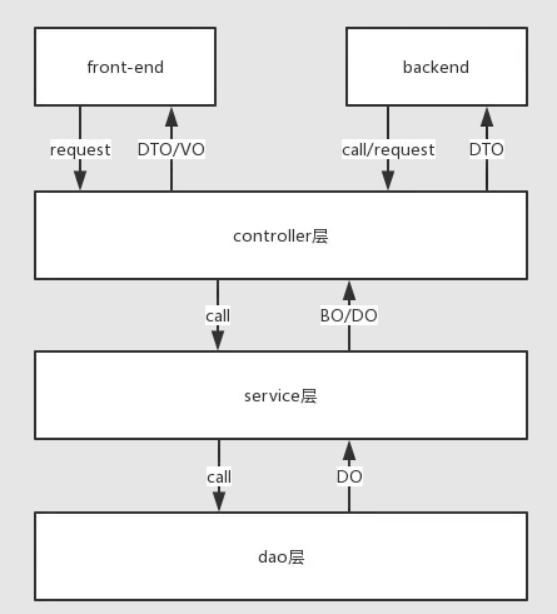
\includegraphics[width=0.5\textwidth]{figures/31.png}
	\caption{代码结构}
\end{figure}

\subsubsection{Controller层}
\begin{itemize}
	\item \textbf{处理HTTP请求}:Controller层接收来自前端的HTTP请求,并根据请求类型(如GET、POST、PUT、DELETE)和请求的资源路径来执行相应的操作。
	
	\item \textbf{提取和验证数据}:从HTTP请求中提取必要的数据,并对其进行验证,确保数据的合法性和完整性。
	
	\item \textbf{调用业务逻辑}:将提取的数据传递给Service层,由Service层执行具体的业务逻辑处理。
	
	\item \textbf{返回响应}:根据Service层处理的结果,构造合适的HTTP响应并发送回客户端。
	
	\item \textbf{异常处理}:处理请求处理过程中可能发生的异常,并返回适当的错误响应。
\end{itemize}

\subsubsection*{Controller层的UI设计原则}
在用户界面(UI)设计中,Controller层遵循以下原则以提升用户体验:
\begin{itemize}
	\item \textbf{用户控制原则}:确保用户能够通过直观的操作来控制系统,例如,通过简化的导航和清晰的指令来引导用户。
	
	\item \textbf{减轻记忆负担原则}:减少用户需要记忆的信息量,例如,通过使用自动完成、历史记录或提供清晰的指引来减少用户的记忆负担。
	
	\item \textbf{界面一致性原则}:保持界面的一致性,使得用户无论在哪个模块都能有相同的操作体验,例如,使用统一的布局、颜色方案和控件。
\end{itemize}

Controller层的设计旨在为用户提供一个直观、易用且响应迅速的交互界面,同时也确保了系统的灵活性和可维护性。通过精心设计的Controller层,我们的医疗预约管理系统能够提供高效、个性化的服务,满足不同用户的需求,从而提升整体的医疗服务体验。

在医疗预约管理系统的服务器端设计中,Service层扮演着核心角色,负责实现系统的业务逻辑。以下是Service层及其相关层次的详细描述:

\subsubsection*{Service层}
Service层是系统的核心业务逻辑层,它处理用户请求并执行相应的业务逻辑。在这一层中,我们细分了以下模块:

\begin{itemize}
	\item \textbf{事件类}:负责管理所有事件信息,例如预约挂号和健康咨询等医疗服务事件。
	
	\item \textbf{关系类}:建立事件与提醒之间的联系,并定义它们之间的各种关系,如时间或地点的关联。
	
	\item \textbf{提醒类}:规定在特定事件发生时应采取的行动,例如发送通知给用户或启动提醒机制。
\end{itemize}

\subsubsection*{Mapper层(Dao层)}
Mapper层,也称为数据访问对象(Dao)层,是系统的数据访问层。它作为系统与数据库之间的桥梁,提供数据访问接口,使得Service层能够安全、准确地读写数据库中的数据。这一层的存在确保了系统的稳定性和数据的完整性。

\subsubsection*{Model层}
Model层包含了与数据库表字段相对应的实体类。这些实体类封装了数据,并提供了标准的set/get方法,以支持数据的操作和访问。Model层是Service层和Mapper层之间数据交互的媒介。

通过Service层、Mapper层和Model层的协同工作,医疗预约管理系统能够为病人提供以下一站式医疗服务:

\begin{itemize}
	\item 用户注册与登录,确保用户能够安全地访问系统服务。
	\item 查看和管理个人健康信息,提供个性化的医疗信息管理。
	\item AI病情咨询服务,利用人工智能技术为病人提供初步的医疗建议。
	\item 科室选择和医生预约挂号,优化就诊流程,提高医疗服务的可及性和效率。
\end{itemize}

系统还支持电子问诊单的接收,便于病人记录和后续跟进,确保医疗服务的连续性。此外,病人可以通过参与医疗服务评价体系,为医疗服务提供宝贵的反馈,帮助医疗机构不断改进服务质量。

在技术实现方面,项目采用了面向对象的设计原则,前端框架的构建是开发团队的主要责任。我们选择了Vue.js作为前端框架,并使用JavaScript作为编程语言,以实现高效、响应式的用户界面。

总体而言,这些功能的实现旨在为病人提供一个无缝、高效的医疗服务体验。通过提升医疗服务的可及性和效率,这些设计不仅满足了病人的需求,也为医疗服务的整体改进和发展做出了重要贡献。

在医疗预约管理系统的服务器端设计中,除了核心的业务逻辑层和服务层之外,还需要考虑数据的安全性和稳定性。以下是数据备份与恢复以及安全性保障的详细描述:

\subsubsection*{数据备份与恢复}
为了确保系统的稳定性和数据的安全性,服务器软件必须提供可靠的数据备份和恢复机制。这一机制的重要性体现在以下几个方面:

\begin{itemize}
	\item \textbf{故障恢复}:在软硬件故障发生时,系统必须能够利用备份的数据迅速恢复运行环境,以减少系统停机时间,保证服务的连续性。
	
	\item \textbf{数据完整性}:用户信息管理模块的安全性至关重要,必须确保用户信息的完整性和准确性,包括个人资料、预约记录、健康信息等。
	
	\item \textbf{统计数据的准确性}:系统应定期进行数据备份,确保在任何时候都能够恢复到一个已知的、准确的数据状态。
\end{itemize}

为了实现这些目标,可以采取以下措施:

\begin{itemize}
	\item 实施定期自动备份策略,包括全量备份和增量备份。
	\item 确保备份数据的存储安全,避免数据丢失或损坏。
	\item 测试备份数据的恢复流程,确保在紧急情况下能够快速有效地恢复数据。
\end{itemize}

\subsubsection*{安全性保障}
安全性是医疗预约管理系统的另一个关键考虑因素。系统应实施以下加密措施来保障数据的保密性和安全性:

\begin{itemize}
	\item \textbf{登录数据加密}:对用户的登录信息,如用户名和密码,进行加密处理,以防止未授权访问。
	
	\item \textbf{传输数据加密}:对在系统间传输的数据进行加密,无论是用户信息还是医疗记录,都应确保在传输过程中不被截获或篡改。
	
	\item \textbf{数据存储加密}:对存储在数据库中的敏感数据进行加密,即使数据被非法访问,也无法直接读取内容。
\end{itemize}

此外,系统还应采取其他安全措施,如:

\begin{itemize}
	\item 实施强密码策略和定期密码更换提醒。
	\item 使用防火墙和入侵检测系统来防止未经授权的访问。
	\item 定期进行安全审计和漏洞扫描,以发现并修复潜在的安全问题。
\end{itemize}

通过这些措施,医疗预约管理系统能够为病人提供一个安全、可靠的医疗服务体验,保护病人的隐私和数据安全,同时也符合医疗行业的安全标准和法规要求。